\documentclass[letterpaper,10pt]{article}
\usepackage{fullpage}
\usepackage{times}
\usepackage{cite}
\usepackage{fancyvrb}
\usepackage{moreverb}
\usepackage{graphicx}
\usepackage{hyperref}

\newcommand{\squishlist}{\begin{list}{$\bullet$}
  {\setlength{\itemsep}{0pt}
    \setlength{\parsep}{3pt}
    \setlength{\topsep}{3pt}
    \setlength{\partopsep}{0pt}
    \setlength{\leftmargin}{1.5em}
    \setlength{\labelwidth}{1em}
    \setlength{\labelsep}{0.5em}}}

\newcommand{\squishend}{\end{list}}

\title{CS8803SS, Spring 2010, Project Proposal}
\author{
  Jason Rodzik and Nick Black
}
\date{}

\begin{document}
\maketitle

\section{Introduction}
Heterogeneous computing has definitely arrived, and GPGPU units in the millions
are employed worldwide. Tradition has shown newly programmable domains to be
rapidly subjected (and often found vulnerable) to attacks of the past; indeed,
wherever processing goes, so does the possibility of automated attacks. With
high powered GPU's moving from the gamer's desktop to the laboratory's cluster,
it's essential that the security issues surrounding their use be fleshed out
earlier rather than later. Unfortunately, this is not the case; graphics card
manufacturers have not publicized any of their own internal security studies
(if any exist), and popular manufacturers are infamous for their
hostility to open source and academia\footnote{See for instance Wikipedia's page on
``\href{http://en.wikipedia.org/wiki/NVIDIA\_and\_FOSS}{Graphics hardware and FOSS}''.}
We suspect that existing GPGPU platforms from NVIDIA and ATI are already
susceptible to certain attacks. We furthermore expect to develop defenses to
these attacks. We hope to discover new, bold, even savage attacks on
the GPGPU paradigm---or, perhaps prove that such unexpected results are impossible.

\section{Goals}
We will perform a comprehensive analysis of the security issues surrounding
general purpose graphics processing units and computations in which they are
involved. We will begin from the theoretical direction, using Bishop's taxonomy
to describe the possible threat space. The hardware and software interfaces will
be investigated, enumerated, and analyzed regarding their potential relevance
to this set of possible issues (work here will likely proceed well past the
open literature, and consume most of the project's time). Any definite problems
or solutions will be closely detailed, in prose and code both. Defenses will 
be implemented through the proof-of-concept stage, and attacks at least crudely
weaponized.

\section{Related work}
Our research in this area is focused on the possibility of security
vulnerabilities against the GPU itself, an area which we were unable to find
prior research for. However, our research is motivated in part by an increase
in applications being developed for GPUs and also by GPUs being used as the
processing unit for security related tasks.
  
\subsection{General applications}
  
  Dedicated graphical processing units (GPUs) have seen significant advancement
in the past couple decades due to the insatiable demand that consumers have for
ever-increasing advances in video game graphics. This development has led to
recent GPUs reaching the point where they are powerful enough that there has
been significant research invested into using them to execute tasks outside the
realm of video games. One of the most popular examples of this is the
Folding@Home project, which in recent years has developed a version of its
application that runs on both ATI and nVidia brand GPUs
\url{http://folding.stanford.edu/English/Guide#ntoc4}.
  
  In 2007, nVidia released the SDK for CUDA, their "Compute Unified Device
Architecture," allowing for the GPU to be much more accessible to developers
wishing to use the GPU for non-graphical applications. In the three years since
then, a wide variety of applications for CUDA have been developed\footnote{\url{http://www.nvidia.com/object/what\_is\_cuda\_new.html}}.
  
  General Mills developed an application that used CUDA to model the optimal
way to cook a frozen pizza in a microwave. SeismicCity used CUDA to improve the
amount of time it takes to interpret seismic data to determine the optimal
drilling locations for finding oil
\url{http://www.nvidia.com/object/cuda\_in\_action.html}.
  
  Other companies are offering CUDA solutions for problems in the realms of
electromagnetics, bioinformatics, finance, accelerator physics, aerodynamics,
engine optimizations, image and video stream compression, healthcare and life
sciences, medical imaging, defense, and more
\squishlist
\item \url{http://www.acceleware.com/default/index.cfm/professional-services/}
\item \url{http://www.aneo.fr/index.php?option=com\_content&amp;view=article&amp;id=91&amp;Itemid=110}
\item \url{http://www.parallel-compute.com/}
\item \url{http://www.caps-entreprise.com/nvidia.html}
\item \url{http://www.elegant-mathematics.com/index.html?NVGPU}
\item \url{http://www.culatools.com/consulting}
\item \url{http://www.fixstars.com/en/solutions/gpu/}
\item \url{http://www.hoopoe-cloud.com/Services.aspx}
\item \url{http://www.hpc-project.com/gpu2.htm}
\item \url{http://www.sagivtech.com/21541.html}
\item \url{http://www.stoneridgetechnology.com/services/visualcomputing.asp}
\item \url{http://gpucomputing.txcorp.com/}.
\squishend
  
\subsection{Security applications}
  There are a few research areas where GPUs have been used in security applications, but all of these involve using the GPU as a faster processor than the CPU, and none of the research involves investigating the GPU itself or coding frameworks such as CUDA from a security standpoint.
  
  The most common security task that GPUs have been used for in prior work have been to use the GPU for performing cryptographic computations. Research has found that GPUs can perform some AES-related OpenSSL computations up to 20 times as fast as a typical implementation
\url{http://www.manavski.com/downloads/PID505889.pdf}. Another aspect that is of importance, particularly to copyright groups such as the RIAA and MPAA, are the encryption techniques used with GPUs for the security of applications involving remote displays, such as for HDCP blu-ray implementations\url{http://www.amazon.com/CryptoGraphics-Exploiting-Graphics-Security-Information/dp/038729015X}.
  
  While GPUs can be used for improving the speed of cipher implementations, they can be used to speed up cryptographic attacks as well. In some cases, applications have been developed using CUDA to allow for WiFi keys to be broken up to 100 times as fast as in typical implementations \url{http://arstechnica.com/security/news/2008/10/company-puts-nvida-gpus-to-work-cracking-wireless-security.ars}.
  
  Intrusion detection systems can exhibit performance degradation under heavy
  loads, and some of the proposed solutions to this problem have involved
  offloading IDS computations to the GPU
  \url{http://citeseerx.ist.psu.edu/viewdoc/download?doi=10.1.1.125.3302&amp;rep=rep1&amp;type=pdf}.
  Additionally, some techniques in pattern-matching are difficult to perform
  quickly enough to be useful, and GPUs have been proposed as a solution that
  allow for significant decreases in computation time
  \url{http://portal.acm.org/citation.cfm?id=1395492}.


\section{Plans}

We will work axiomatically, first asserting the space of interfaces, and then
performing a breadth-first search through its marrow. This will likely involve
significant reverse engineering of the closed-source NVIDIA drivers, differential
analysis across their revision histories, and attempts to acquire restricted
documentation. NVIDIA's dumpsters being regrettably distant, this last will be
largely restricted via social engineering, speculative (but not penetrative)
search, and consultation of peer-to-peer file-sharing networks.

Further work will proceed from there.

\section{Timeline}
In the time we have between now and the first deliverable we will be conducting exploratory research to determine the possible areas of interest in CUDA as it relates to software security. We will then allow ourselves a few days to prepare our intermediate paper submission before continuing on our research. The next phase of our research will involve focusing on at least one specific area of interest that was identified in the initial research phase, at which point we will identify all possible security issues for the given area and determine the scope of these issues. Finally, we will allow ourselves time to write our final paper before preparing and practicing our presentation and conducting any final, last-minute research before the final presentation.

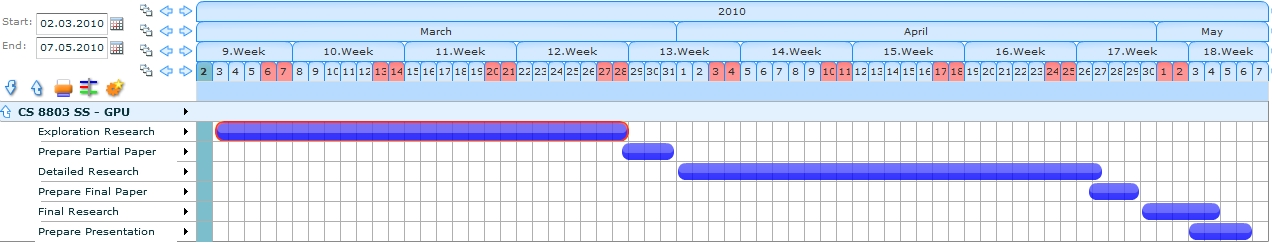
\includegraphics[width=\columnwidth]{texobjs/dstvt2g_6d5trvxfm_b.jpg}
%  <img height=197 src="
%" width=1032>
\end{document}
